\documentclass[a4paper,10pt]{article}
\usepackage{hyperref}
\usepackage{setspace}
\usepackage{graphicx}
\usepackage{color}
\usepackage{xcolor}
\usepackage{relsize}
\usepackage{listings}
\usepackage[round]{natbib}
\usepackage{minted}
\usepackage{float}
\hypersetup{colorlinks = true, linkcolor = blue, citecolor = black}
\lstset{language=Python}
\usepackage[margin=0.75in]{geometry}

\usepackage{listings}
\usepackage{makeidx}
\usepackage{titlesec}
\setcounter{tocdepth}{5}
\usepackage[T1]{fontenc}
\usepackage[utf8]{inputenc}
\usepackage{authblk}
\makeindex{}
%\VignetteEngine{knitr}
%\VignetteIndexEntry{A Markdown Vignette with knitr}
\definecolor{bg}{rgb}{0.95,0.95,0.95}


\title{\textbf{A bioinformatics workflow for detecting signatures of selection in genomic data}}
\date{December 12, 2013}

\author[1]{Murray Cadzow}
\author[1]{James Boocock}
\author[1,2]{Hoang Tan Nguyen}
\author[1,3]{Phillip Wilcox}
\author[1]{Tony R Merriman}
\author[1]{Michael A Black}
\affil[1]{Department of Biochemistry, University of Otago}
\affil[2]{Department of Mathematics and Statistics, University of Otago}
\affil[3]{Scion Research, Rotorua, New Zealand}
\renewcommand\Authands{ and }
\begin{document}

\maketitle{}\textmd{}
\spacing{1.5}
%\doublespacing
\tableofcontents

\pagebreak
\section{Introduction}

This selection analysis workflow utilizes genotype data derived from
next-generation sequencing (NGS) or high-denisity microarray (e.g.,
``SNP chip'') experiments to identify the presence of signatures of
selection. The tools used to detect selection are dependent on the
selection signature being investigated \citep{Sabeti:2006ha}. The
pipeline presented here generates various output files containing
within- and between-population selection signatures. The starting
point for the analysis
is a variant call format (VCF) file of the genotype data and
populations of interest \citep{Danecek:2011gz}. Both $F_{ST}$ and
Tajima's D can be calculated from standard genotype data
\citep{Weir:1984vn, Tajima:1989un}. To compute iHS, Rsb and Fay
and Wu's H requires haplotype information, and thus the genotype data must be
phased prior to calculation of these statistics \citep{Voight:2006go,
  Gautier:2012et,fayandwush}. For phasing, shapeit2 is
used, and for imputation impute2 is used \citep{impute22009,
  Delaneau:2013hi}. Furthermore these statistics also require
ancestral allele information \citep{Flicek:2012vg}.  The pipeline
performs phasing if the VCF files do not contain phase information, and
then performs ancestral allele annotation. 
{\bf\color{blue}\small [*** JAMES - IS THIS ONLY TRUE FOR HUMAN DATA?  ***]}
Once complete, the rehh
package for R provides a simple interface for implementing EHH-based
analyses \citep{Gautier:2012et}. Here we have extended rehh to include penalties
for gaps that match those used in the original iHS paper
\citep{Voight:2006go}. rehh is used to calculate iHH, iHS, iES and Rsb. To
calculate Fay and Wu's H, a C program, variscan, was utilised
\citep{variscan2005}. The pipeline is implemented in Python, and takes a VCF
file as input. The output is a colection of files relating to selection
signatures dected by the various software tools.

\section{Getting Started}
\subsection{Prerequisites}
The selection pipeline was developed on a 64-bit Ubuntu 13.04 system
and has been tested on 64-bit Centos and Ubuntu 13.10
installations. The pipeline should work on any 64-bit linux derivative
assuming some basic libraries and tools are installed on the
system. 8GB of RAM should be sufficient for all computation steps
(imputation is the most RAM-intensive component of the pipeline).

\begin{itemize}
\item Python > = 2.6 
\item Bourne-again Shell (Bash)
\item Perl5
\item R \( >= 3.0.0 \) (with the ability to install packages into a
  library within your home directory structure)
\item GNU Autotools
\item GCC 
\item Git
\end{itemize}
The software is installed with the same permissions as the user than
runs the script: if the user is not root then a local (i.e.,
user-writeable) R library is
required. The program also installs the scripts to the user's
~/.local/bin directory.  This directory should be added to the system
PATH to give direct access to the programs from the command-line. 
 
\subsection{Python dependencies}
The following Python packages are required for the pipeline:
\begin{itemize}
\item python-setuptools
\item python-numpy
\item python-scipy

if using python < 2.7 the package argparse will need to be installed.

It can be installed using the following command.

\begin{minted}[bgcolor=bg,frame=lines]{bash}
easy\_install-2.6 argparse
\end{minted}
\end{itemize}
Most linux distributions provide these packages through the official
package management repositories.
\subsection{Downloading}
The selection pipeline can be obtained at the url:
\href{https://github.com/smilefreak/selectionTools}
{https://github.com/smilefreak/selectionTools}

\noindent
To download run the following command in a terminal.

\begin{minted}[bgcolor=bg,frame=lines]{bash}
git clone https://github.com/smilefreak/selectionTools
\end{minted}

\subsection{Installation}

\noindent
To perform an automatic installation of the selection
analysis pipeline, run the following command in the root of the
directory in which the pipeline was installed (i.e., within the
``selectionTools'' directory).\\
\begin{minted}[bgcolor=bg,frame=lines]{bash}
./install.sh
\end{minted}

\noindent
The installation process creates a default configuration file located in the base
directory of the pipeline. It also adds a program called
selection\_pipeline to the system path. To test that the program is
installed correctly, run the following command at a terminal prompt.

\begin{minted}[bgcolor=bg,frame=lines]{bash}
selection_pipeline -h
\end{minted}

\noindent
If the above command does not work, make sure that ~/.local/bin/ is included in the PATH environment variable.

\subsection{Genetic Maps and Impute Haplotypes}
To use the phasing and imputation features of the pipeline requires
both genetic map files and haplotype files. For humans, files
that conform to the format required for shapeit and impute2 can be
found
\href{http://mathgen.stats.ox.ac.uk/impute/impute_v2.html#reference}{here}. For
impute2, one reference is available
\href{http://mathgen.stats.ox.ac.uk/impute/ALL_1000G_phase1integrated_v3_impute_macGT1.tgz}{here}.
Download and extract the archive to referencefiles/impute\_ref and
uncompress the contents. For shapeit2, a genetic map can be found
\href{http://www.shapeit.fr/files/genetic_map_b37.tar.gz}{here}.
Download and extract the archive to referencefiles/shapeit\_ref.\\


To use other reference files with the selection pipeline requires
setting the following options in the config file. The question mark character
"?" in the config is substituted by the chromosome number: this is
used for reference files that are split on chromosomes.\\


\begin{minted}[bgcolor=bg,frame=lines]{bash}
...
genetic_map_prefix=genetic_map_chr?_combined_b37.txt
...
impute_map_prefix=genetic_map_chr?_combined_b37.txt
impute_reference_prefix=ALL_1000G_phase1integrated_v3_chr?_impute
...
\end{minted}

\noindent
If you decide to store the reference files in another location,
further options require alteration in the config file:\\ 
\begin{minted}[bgcolor=bg,frame=lines]{bash}
...
genetic_map_dir= ${HOME}/MerrimanSelectionPipeline/referencefiles/shapeit_ref
...
impute_map_dir= ${HOME}/MerrimanSelectionPipeline/referencefiles/impute_ref
impute_reference_dir= \${HOME}/MerrimanSelectionPipeline/referencefiles/impute_ref
...
\end{minted}

\subsection{Ancestral Fasta Files}
The generation of results for iHS requires assigning the ancestral
allele. The selection pipeline uses the ancestral alleles from the
6-way EPO (Enredo-Pecan-Ortheus) alignment pipeline. The files can be
downloaded from
\href{ftp://ftp.1000genomes.ebi.ac.uk/vol1/ftp/phase1/analysis_results/supporting/ancestral_alignments/human_ancestor_GRCh37_e59.tar.bz2}{here}. Be
sure to extract the contents of the archive after download. The default
directory to store the ancestral reference files is\\
\begin{minted}[bgcolor=bg,frame=lines]{bash}
referencefiles/ancestral_ref/
\end{minted}

\noindent
If you downloaded your reference to a different location you can alter the following setting in your config file.\\
\begin{minted}[bgcolor=bg,frame=lines]{bash}
...
ancestral_fasta_dir = # directory you downloaded alignment to #
...
\end{minted}

\section{Tutorial}
\subsection{Selection Signatures at the Lactase Locus}
\subsubsection{Getting the Data}
In humans, lactase is encoded by the LCT gene, which is located on
Chromosome 2 at the coordinates:
136,545,410-136,594,750. For this example we will use a 10
megabase region containing the LCT, and genotype data from the CEU and YRI
populations from the 1000 Genomes Project. In order to demonstrate the
functionality of the pipeline we will use the chromosome 2 region
130,000,000-140,000,000. The lactase gene is an example of strong selection in
the last 5,000-10,000 years in human populations, specifically
those of European ancestory \citep{lactase2004}. The tutorial commands will be given as examples using phasing and imputation or taking advantage of the fact that the 1000 genomes VCF files actually contain phasing information. If you choose to run the tutorial without using phasing and imputation you will only need to download the Ancestral allele information.
To download the example dataset enter the following command:

{\small
\begin{minted}[bgcolor=bg]{bash}
git clone https://github.com/smilefreak/SelectionPipelineTestData
\end{minted}
}

\noindent
Navigate to the created SelectionPipelineTestData folder and extract \emph{selection\_pipeline\_tutorial.tar.gz}. 

\begin{minted}[bgcolor=bg,frame=lines]{bash}
cd SelectionPipelineTestData
tar xzf selection_pipeline_tutorial.tar.gz
\end{minted}

\subsection{Setting up the Pipeline Run}
\subsection{Population Files}
Population files are required for any cross population
comparisions. The commands below will initiate the data generation
step. Population files are line seperated files, where the first line
contains the population name, and every successive line contains an
individual ID from that population.\\

\begin{minted}[bgcolor=bg,frame=lines]{bash}
<POPULATION_IDENTIFIER>
<INDIVIDUAL ID 1>
<INDIVIDUAL ID 2>
.......
<INDIVIDUAL ID N>
\end{minted}
\subsection{Run The Tutorial}
The default configuration file is located in the base directory of the
selection pipeline. To run the pipeline with phasing and imputation, execute the command below in the folder in which the example data were extracted, and change the
--config-file parameter to match the location where the pipeline is installed.\\
\begin{minted}[bgcolor=bg,frame=lines]{bash}
multipop_selection_pipeline -p CEU_ids.txt -p YRI_ids.txt \
  -i CEU_YRI_lactase.vcf --config-file defaults.cfg \
  -a "--imputation"
\end{minted}

\noindent
As the 1000 genomes datasets are actually phased VCF to run the pipeline without phasing run the following command. The --phased-vcf option significantly speeds up the selection pipeline.

\begin{minted}[bgcolor=bg,frame=lines]{bash}
multipop_selection_pipeline -p CEU_id.txt -p YRI_ids.txt \
    -i CEU_YRI_lactase.vcf --config-file defaults.cfg \
    --a "--phased-vcf"    
\end{minted} 

\noindent
The generated folders and current folder have all the data required to
perform further selection analysis. Within each population folder four
output files are generated.  These contain Tajima's D, iHH, an updated
VCF, and Fay and Wu's H statistic. The files are located in the
results folder inside each population subfolder. $F_{ST}$ is calculated
between each population and results are located in the fst folder. $F_{ST}$
results are calculated using the Weir and Cockerham estimator.

\subsection{Data Visualisation}
The purpose of the analysis pipeline is to generate standard signatures of
selection from a VCF formatted input file. In order to assist with
exploring/interpretting the results, visualization of the pipeline
output can be extrenely useful.
%In order to express the
%usefulness of the pipeline it is pertinent to illustrate the
%effectiveness of the pipeline. 
The next section describes some basic approaches to 
plotting these data using the R programming language. All of the following
commands are run in an R session with the working directory set as the base
directory from which the tutorial is being run. In each of the plots
that follow, the vertical blue lines indicate the position of the
lactase gene (LCT).

\subsubsection{Visualizing $F_{ST}$ values}

\noindent
Plot the $F_{ST}$ results across the entire 10 megabase region for the tutorial.  Mean $F_{ST}$ is being plotted in each case.\\

\noindent
Plot mean Weir FST values.\\
\begin{minted}[bgcolor=bg,frame=lines]{r}
weirFST = read.table('fst/2CEUYRI.weir.fst',header=T) 
plot(weirFST[,6]~ weirFST[,2], pch=16, cex=.4, 
type="p",ylab=expression(F[ST]),xlab="Chromosome position (bp)") 
abline(h=mean(weirFST[,6]) + 3 * sd (weirFST[,6]),col='red')
rect(136545410,-1900,136594750,100,border="Blue") 
\end{minted}

\begin{figure}
\centering
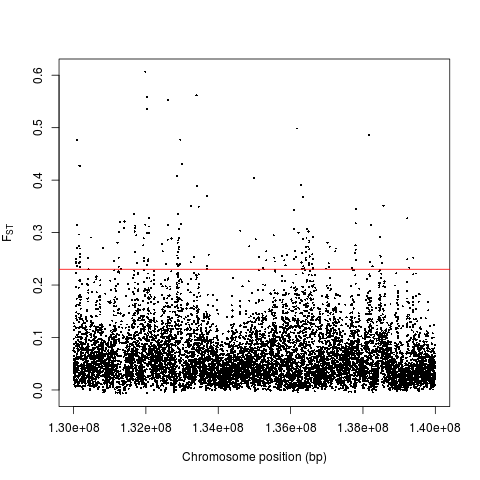
\includegraphics{pictures/WeirCEUYRI.png}
\caption{Values of Weir $F_{ST}$ mean FST between the CEU and YRI populations}
\label{fig:a}
\end{figure}

\noindent
Plot mean HapMap FST values.\\
\begin{minted}[bgcolor=bg,frame=lines]{r}
hapmapFST = read.table('fst/2CEUYRI.hapmap.fst',header=T) 
plot(hapmapFST[,6]~ hapmapFST[,2], pch=16, cex=.4, 
type="p",ylab=expression(F[ST]),xlab="Chromosome position (bp)") 
abline(h=mean(hapmapFST[,6]) + 3 * sd (hapmapFST[,6]),col='red')
rect(136545410,-1900,136594750,100,border="Blue") 
\end{minted}
\begin{figure}
\centering
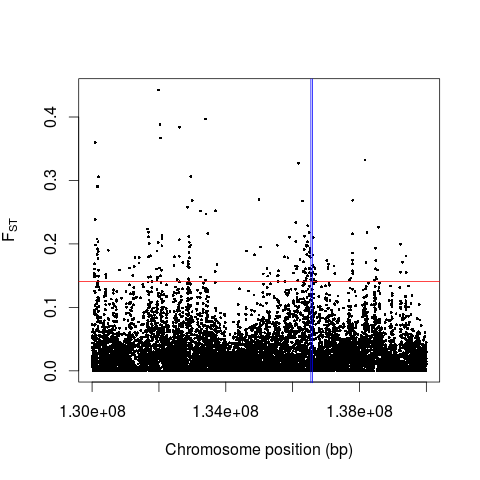
\includegraphics{pictures/hapmapCEUYRI.png}
\caption{Values of HapMap $F_{ST}$ mean FST between the CEU and YRI populations}
\label{fig:hapmapfst}
\end{figure}

\noindent 
Figures (~\ref{fig:a} and ~\ref{fig:hapmapfst}) show the weir and hapmap FST values for the tutorial region.

\subsubsection{Fay and Wu's H}
Plot the Fay and Wu's H values for the CEU population:\\
\begin{minted}[bgcolor=bg,frame=lines]{r}
CEUFay=read.table('CEU/results/CEU2.faw',comment.char="#")
#Plot Fay and Wu's H
plot(CEUFay[,15] ~ CEUFay[,1],xlim=c(136545410-1e6,136594750+1e6),
pch='.',cex=2,ylim=c(-50,0),
xlab='Chromosome position (bp)',ylab="H Statistic")
rect(136545410,-1000,136594750,100,border="Blue") 
\end{minted}
\begin{figure}
\centering
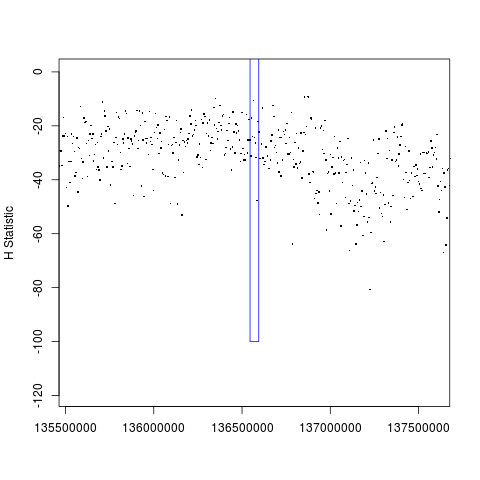
\includegraphics{pictures/CEUFay.png}
\caption{Fay and Wu's H statistic in the CEU population, across a two
  megabase region around the LCT gene.}
\label{fig:fayceu}
\end{figure}

\noindent
Figure~\ref{fig:fayceu} shows the Fay and Wu's H statistic one
megabase downstream and upstream of the lactase gene.  Plot the Fay
and Wu's H values for the YRI population:\\
\begin{minted}[bgcolor=bg,frame=lines]{r}
YRIFay=read.table('YRI/results/YRI2.faw',comment.char="#")
#Plot Fay and Wu's H
plot(YRIFay[,15] ~ YRIFay[,1],xlim=c(136545410-1e6,136594750+1e6),pch='.',cex=2,ylim=c(-50,0),
xlab='',ylab="H Statistic")
rect(136545410,-1900,136594750,100,border="Blue") 
\end{minted}
\begin{figure}
\centering
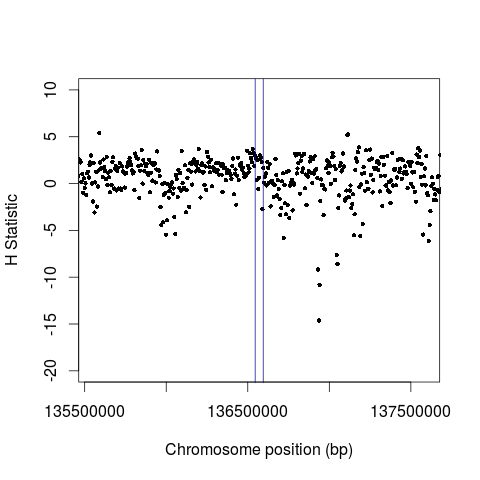
\includegraphics{pictures/YRIFay.png}
\caption{Fay and Wu's H statistic in the YRI population, across a two
  megabase region around the LCT gene.} 
\label{fig:fayyri}
\end{figure}

\noindent
Figure~\ref{fig:fayyri} shows Fay and Wu's H statistic one megabase
downstream and upstream of the lactase gene.

\subsubsection{iHS}
Plot the iHS values around the lactase gene for the CEU population:\\
\begin{minted}[bgcolor=bg,frame=lines]{r}
CEUihs = read.table('CEU/results/CEUchr2.ihs')
#plot IHS pvalues
plot(CEUihs[,4] ~ CEUihs[,2],xlim=c(1.364e8,1.368e8),pch='.',cex=2,
ylab=expression("-" * log[10] * "[" ~ "1-2|" * Phi[scriptstyle(italic(iHS))] * "-0.5|" ~ "]"),
xlab="Chromosome Position BP") 
rect(136545410,-10,136594750,10,border="Blue") 
abline(h=2,col="red")
\end{minted}

\begin{figure}
\centering
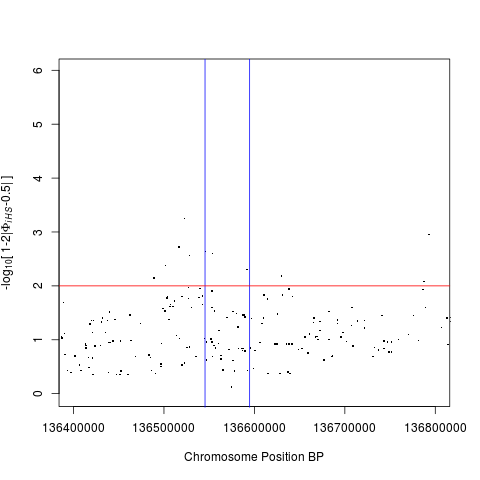
\includegraphics{pictures/CEUihs.png}
\caption{iHS statistic in the CEU population, across a 400 kilobase region around the LCT gene. }  
\label{fig:ceuihs}
\end{figure}

\noindent
Figure ~\ref{fig:ceuihs} shows iHS pvalues around the lactase gene in the CEU population.

\noindent
Plot the iHS values around the lactase gene for the YRI population:\\
\begin{minted}[bgcolor=bg,frame=lines]{r}
YRIihs = read.table('YRI/results/YRIchr2.ihs')
#plot IHS pvalues
plot(YRIihs[,4] ~ YRIihs[,2],xlim=c(1.364e8,1.368e8),pch='.',cex=2,
ylab=expression("-" * log[10] * "[" ~ "1-2|" * Phi[scriptstyle(italic(iHS))] * "-0.5|" ~ "]"),
xlab="Chromosome Position BP") 
rect(136545410,-10,136594750,10,border="Blue") 
abline(h=2,col="red")
\end{minted}

\begin{figure}
\centering
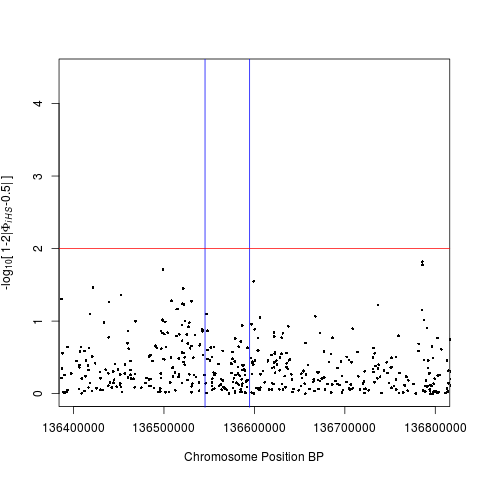
\includegraphics{pictures/YRIihs.png}
\caption{iHS statistic in the YRI population, across a 400 kilobase region around the LCT gene. }
\label{fig:yriihs}
\end{figure}

\noindent
Figure ~\ref{fig:yriihs} shows iHS pvalues around the lactase.

To visualize individual SNPs, a haplotype bifurication diagram can be
used \citep{Gautier:2012et}. The SNP rs28453840 displayed a strong signal of
selection using iHS in the CEU population. The following commands construct a bifurcation diagram for both
alleles at this SNP using rehh. \\

\noindent

\begin{minted}[bgcolor=bg,frame=lines]{r}
# Plot  bifurcation diagram.
load('CEU/results/CEUchr2.RData')
par(mfrow=c(2,1))
bifurcation.diagram(haplohh=d,mrk_foc=13750,all_foc=1)
bifurcation.diagram(haplohh=d,mrk_foc=13750,all_foc=2)
\end{minted}
\begin{figure}
\centering
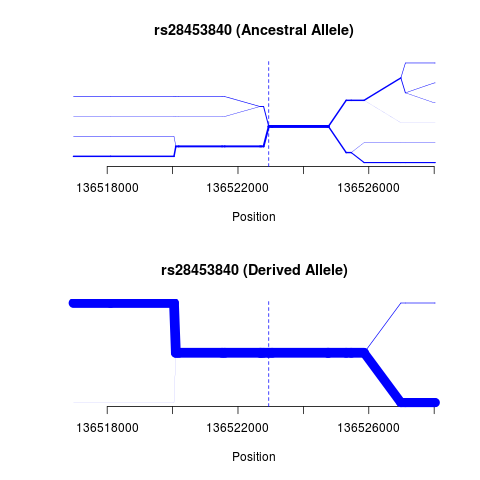
\includegraphics{pictures/bifurcationCEU.png}
\caption{Bifurcation Diagram for rs28453840}
\label{fig:bifurcationceu}
\end{figure}

\noindent
Figure ~\ref{fig:bifurcationceu} shows the bifurcation plot for rs28453840 a snp that had a iHS score greater that 3 at position 136522941 on chromosome 2 just upstream of lactase.

\subsubsection{Tajima's D}

\begin{minted}[bgcolor=bg,frame=lines]{r}
tajimaD=read.table(file="CEU/results/CEU2.taj_d", header=TRUE)
plot(tajimaD[,4] ~ tajimaD[,2],pch='.',cex=2,xlab="Chromosome position (bp)", ylab="D statistic")
rect(136545410,-10,136594750,10,border="Blue") 
\end{minted}

\begin{figure}
\centering
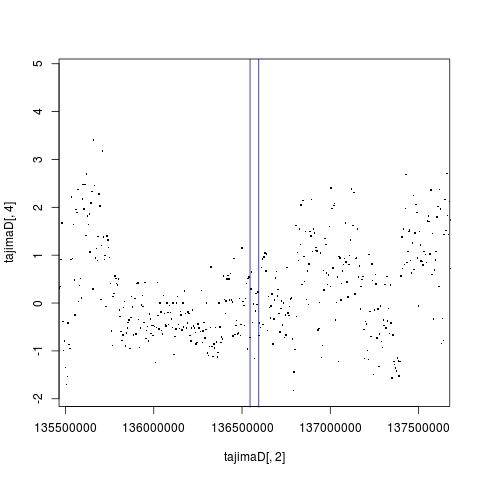
\includegraphics{pictures/CEUtajimas.png}
\caption{Tajima's D statistic in the CEU population, across the full 10 megabase pipeline region.}
\label{fig:tajceu}
\end{figure}

\noindent
Figure~\ref{fig:tajceu} show the Tajima's D statistic across the full tutorial region.

\begin{minted}[bgcolor=bg,frame=lines]{r}
tajimaD=read.table(file="YRI/results/YRI2.taj_d", header=TRUE)
plot(tajimaD[,4] ~ tajimaD[,2],pch='.',cex=2,xlab="Chromosome position (bp)", ylab="D statistic")
rect(136545410,-10,136594750,10,border="Blue") 
\end{minted}

\begin{figure}
\centering
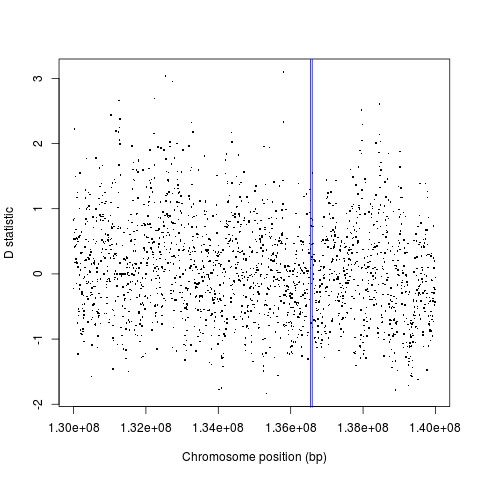
\includegraphics{pictures/YRItajimas.png}
\caption{Tajima's D statistic in the YRI population for the tutorial region} 
\label{fig:tajyri}
\end{figure}

\noindent
Figure~\ref{fig:tajyri} show the Tajima's D statistic across the full tutorial region.

\subsubsection{Rsb}

Rsb makes the differeneces between the two populations very clear. The following code shows how to plot the Rsb bilateral P-values for the 10 megabase tutorial region.
\noindent
\begin{minted}[bgcolor=bg,frame=lines]{R}
rsb = read.table('rsb/2CEUYRI.rsb',header=T)
plot(rsb[,4] ~ rsb[,2],pch='.',cex=2)
abline(h=2,col='red')
# Plotting the lactase gene.
rect(136545410,-10,136594750,10,border="Blue")
\end{minted}

\begin{figure}
\centering
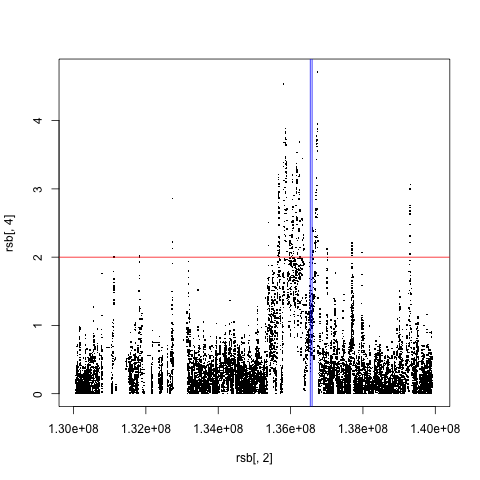
\includegraphics{pictures/RSBCEUYRI.png}
\caption{RSB statistic between the CEU and YRI population for the tutorial region} 
\label{fig:rsb}
\end{figure}
Figure ~\ref{fig:rsb} shows the Rsb statistic for the entire region for the tutorial, it is visually striking the difference at the LCT locus.

\pagebreak
\section{Output Files}
The output files are preserved in the same state as the original output from the program used to generate the data.
\subsection{multi\_population}
\subsubsection{Fst}
Located in the fst folder. Tab-delimited data file containing 1 header line followed data on each subsequent line\\
\begin{minted}[bgcolor=bg,frame=lines]{rst}
CHROM   BIN_START       BIN_END N_VARIANTS      WEIGHTED_FST    MEAN_FST  
2       130000001       130010000       94      0.133102        0.0680276 
\end{minted}
\subsection{selection\_pipeline}
All the outputs for each population are contained in the results folder. If you ran the tool using \emph{multi\_population} the outputs are located in <pop name>/results. 
\subsubsection{Fay and Wu's H}
Space-delimited data file containing header line that start with a hash character (\#). Contains lots of columns. If you are only interested in Fay and Wu's H, column 1 provides the position and column 15 provides the H statistic. \\
\begin{minted}[bgcolor=bg,frame=lines]{rst}
# RefStart   Refend ... FayWu_H
130000040 130005039 ... -22.2438460
\end{minted}
\subsubsection{iHS}
Space-delimited data file containing one header line followed by data on each subsequent line.\\
\begin{minted}[bgcolor=bg,frame=lines]{rst}
"CHR" "POSITION" "iHS" "Pvalue"
"rs4662641" 2 130000272 0.0644902912148128 0.0229261107107533
\end{minted}
\subsubsection{iHH}
Space-delimited data file containing one header line followed by data on each subsequent line.\\
\begin{minted}[bgcolor=bg,frame=lines]{rst}
"CHR" "POSITION" "FREQ_a" "IHHa" "IHHd" "IES"
"rs1251176" 2 130000040 0.9823 11558.89 83915.49 11571.13
\end{minted}
\subsubsection{Tajima's D}
Space-delimited data file containing one header line followed by data on each subsequent line.\\
\begin{minted}[bgcolor=bg,frame=lines]{rst}
CHROM   BIN_START       N_SNPS  TajimaD
2       130000000       22      0.775224
\end{minted}

\section{Command line Arguments}
The selection pipeline contains three programs:
\emph{selection\_pipeline}, \emph{aa\_annotate} and
\emph{multi\_population}. The selection pipeline does all the
intra-population statistics calculations. The multi\_population program
calculates all the inter-population statistics and calls the selection
pipeline. The aa\_annotate program annotates a haplotype file or a
phased vcf file with the ancestral allele from the 6-way EPO
alignment, for other species or alternative ancestral annotation, the
feauture will be added in the future.

\subsection{Multipopulation}
\subsubsection{Input Files}
\begin{itemize}
\item -i <vcf input file>
VCF file containing all the populations you want to analyse from one chromosome or a part of a chromosome only. 
\end{itemize}
\subsubsection{Output Files}
\begin{itemize}
\item FST \\
Fst results are stored in the fst folder with the chromosome number followed by the two populations. e.g 2CEUYRI.fst
\item Selection Pipeline Results\\
All single population pipeline results are stored in the subdirectory of the population in a folder named results. These contain the iHH, Tajima's D and a population VCF file.
\end{itemize}
\subsubsection{Other parameters (Compulsory)}
\begin{itemize}
\item -l <log\_file> \\
Name for the log file. Moved into the logs folder at the end of program run.
\item -c <Chromosome>\\
Integer for the chromosome being used.
\item -a <Arguments to the selection pipeline>\\
Quoted string containing any extra arguments to the selection\_pipeline program. e.g "--imputation"
\item --config-file <path to config file>\\
Path to the selection pipeline config file an example config file is located in the base directory of the extracted package.
\end{itemize}
\subsubsection{Other parameters (Optional)}
\begin{itemize}
\item --no-clean-up\\ 
Do not clean up intermediate data files.
\item --fst-window-size <FST window size>\\
Fst calculation sliding window size in kilobases (default = 1kb).
\item --fst-window-step <FST window step>\\
Fst calculation windoow jump in kilobases, if window size is equal to
the jump size non-overlapping windows are used (default = 1kb).
\item --cores \\
Number of cores avaliable for the pipeline overrides setting in the config file.
\end{itemize}
\subsection{Selection Pipeline}
\subsubsection{Input Files}
\begin{itemize}
\item -i <VCF input file>\\
Single population single chromosome VCF input file. VCf should be unzipped
\end{itemize}
\subsubsection{Output Files}
The Results directory contains all the output files.
\begin{itemize}
\item .ihh file\\
The outputted iHH data for each SNP
\item .taj\_d file\\
Tajima's D output
\item .vcf file\\
Single population VCF updated by the pipeline, can contain.
\end{itemize}
\subsubsection{Other parameters(Compulsory)}
\begin{itemize}
\item --config-file <Config File path>\\
Path to the selection pipeline config file an example config file is
located in the base directory of the extracted package.
\end{itemize}
\subsubsection{Other parameters(Optional)}
\begin{itemize}
\item -l <log\_file> 

Name for the log file. Moved into the logs folder at the end of program run.

\item --maf <minimum MAF>

Minor allele frequency filter threshold any SNPs below this threshold
will be discarded from the analysis (default = 0.01).

\item --hwe <hardy-weinberg minimum p-value>

A hardy weinberg test is performed on every snp any snps failing the
test will be discarded (default = 0.001).

\item --remove-missing <Inclusion threshold for missing genotypes>

Inclusion criteria for SNPs with missing data. SNPs with less than
this value will be removed from analysis (default = 0.99).

\item --fay-Window-Width <window width>

Sliding window width for Fay and Wu's H calculation in kb (default = 5kb).

\item --fay-Window-Jump <Window Jump>

Window jump for Fay and Wu's H calculation, if equal to
fay-Window-Width non-overlapping windows will be used (default =
5kb).

\item --TajimaD <tajimas D bin size>

Tajima's D statistic bin size in kb (default = 5kb).
\item --no-clean-up 

Do not clean up intermediate data files

\item --ehh-window-size

Window size for multicore rehh calculations in megabases (Mb) (default = 5Mb). 

\item --ehh-overlap

Window overlap for multicore rehh calculations in megabases (Mb) (defaut = 2Mb).

\item --daf <Minimum derived allele frequency>

Derived allele frequencies below this minimum will be discarded (default = 0.0).

\item --big-gap

Gap size in kb for not calculating iHH if the gap is too large. If set
to zero the big-gap rule is not applied (default = 0kb).

\item --small-gap

Gap size in kb for applying a penalty to the area calculated by
iHH. If set to zero the small-gap rule is not applied (default = 0kb).

\item --small-gap-penalty

Penalty multiplier for intergration step in iHH
calculation. $multiplier/gap\_size * area$ is the formula we
use. Setting the multiplier to the same value as the small gap
threshold is recommended (default = 0kb).

\item --cores 

Number of cores avaliable for the pipeline overrides setting in the config file. 

\end{itemize}
\subsection{Ancestral Annotation}
The progam \emph{ancestral\_annotation} is installed in the program
path. The program annotates .haps and .vcf files with ancestral allele
annotation from the 6-way IPO alignment or the human reference genome.
\subsubsection{Input Files}
\begin{itemize}
\item -i or --haps <HAPS File>

Haplotype File (.haps)

\item -v <Phased VCF file>

Phased VCF file (.vcf), phased VCF genotypes denoted by a bar ( | ) for each sample.
\item -a or -aa <Ancestral allele fasta>

Ancestral allele annotation file. Currently only works on a the full
1000 Genomes Project GRCh37\.64 reference file or the single chromosome fasta
files from the 6-way EPO alignment.

\end{itemize}
\subsubsection{Output Files}
\begin{itemize}
\item -o or --output <Output file name>

Output file name optional argument by default output is sent to the stdout stream.

\item -s or --sample-file <Sample file output>

Sample file output name ( currently only works with phased vcf option)
\end{itemize}
\subsubsection{Other parameters}
\begin{itemize}
\item --header-regex 

Compulsory argument: it is a regex (regular expression) with a question mark denoting
substitution for the chromosome number. The regex should match the
header in the fasta file and when the question mark is replaced
selectively return only the chromosome of interest. Optional for
single chromosome fasta files.

\item --single-chromosome

Single chromosome pipeline run option.

\item -c <chromosome number>

The number or symbol of the chromosome being used.

\item -f or --format <format>

The 6-way EPO alignment denotes ancestral alleles with both high and
low confidence. To use only ancestral alleles with high confidence use
--format upper. To use both high and low confident alleles use
--format lower. By default the program will use only highly confident
alleles. The highly confident alleles are in uppercase. 

By default it uses all the valid bases in the file that are one  of either A, T, C, G, a, t, c or g

\end{itemize}
\subsection{Configuration File}
The selection pipeline requires a configuration file. By default the
program looks in the current working directory for a file named
defaults.cfg but you can point the program to any file using command
line argument --config-file <config\_file\_location>. There are two
main programs in the selection pipeline namely
\emph{selection\_pipeline} and \emph{multi\_population}. These
programs share a config file but certain configuration parameters can
be ommitted when using the \emph{selection\_pipeline} program
exclusively. A clean install of the pipeline generates an example
configuration file containing default arguments for all the compulsory
parameters. The default config file contains an example of the format.
\subsubsection{system}
\begin{itemize}
\item cores\_avaliable

Certain programs in the pipeline can take advantage of multicore
computers. This option instructs the pipeline about the maximum number
of concurrent processes it is allowed to use.
\end{itemize}
\subsubsection{environment}
\begin{itemize}
\item LD\_LIBRARY\_PATH

Set the library path when running the pipeline, this enables the
pipeline to use the shared libraries that are used for some programs
in the pipeline (alter this option with caution!)

\item PERL5LIB

Sets the PERL5LIB environment variable, this enables the pipeline to
use the perl libraries required by VCFTOOLS (alter this option with
caution!)

\end{itemize}
\subsubsection{selection\_pipeline}
\begin{itemize}
\item selection\_pipeline\_executable

Points to the location of the selection\_pipeline\_executable. 
\end{itemize}
\subsubsection{vcf\_tools}
\begin{itemize}
\item vcf\_tools\_executable 

Points to the vcftools executable, by default it points to the
vcftools executable installed with the pipeline.
\item vcf\_subset\_executable 

Points to the vcf-subset executable, by default pointing to the
vcf-subset installed with the pipeline.
\item vcf\_merge\_executable

Points to the vcf-merge executable, by default pointing to the
vcf-subset installed with the pipeline.
\item extra\_args 

A quoted string containing extra arguments to send to the vcf\_tools executable.
\end{itemize}
\subsubsection{shapeit}
\begin{itemize}
\item shapeit\_executable

Location of the shapeit executable.
\item genetic\_map\_dir 

Directory containing the genetic map for shapeit.
\item genetic\_map\_prefix 

The full file for the genetic map files with a "?" character representing the changing chromosome number.
\item extra\_args 
extra arguments to send to shapeit (Warning: Certain options could
potentially break the pipeline  - use with caution).
\end{itemize}
\subsubsection{impute2}
\begin{itemize}
\item impute\_executable 

Location of the impute2 executable
\item impute\_map\_dir

Directory containing the genetic map for impute2
\item impute\_reference\_dir 

Directory containing the reference panel ( .legend and .hap) files for impute2.
\item chromosome\_split\_size

Window size for imputation calculation.
\item impute\_map\_prefix

The full file name for the genetic map files with a "?" character
representing the changing chromosome number
\item impute\_reference\_prefix

The full file name for the reference panels minus the extension with a
"?" character representing the changing chromosome number.
\item extra\_args

extra arguments to send to impute2 (Warning: Certain options could
potentially break to pipeline use with caution).
\end{itemize}
\subsubsection{plink}
\begin{itemize}
\item plink\_executable 

Location of the plink executable
\end{itemize}
\subsubsection{Rscript}
\begin{itemize}
\item rscript\_executable

Location of the rscript executable (Program usually in path so just Rscript is the default).
\item indel\_filter

Location of the rscript indel\_filter (hap\_indel\_and\_maf\_filter.R)i
\end{itemize}
\subsubsection{haps\_scripts}
\begin{itemize}
\item haps\_to\_hapmap\_script 

Location of the haps\_to\_hapmap script

\item haps\_filter\_script

Location of the haps\_filter script

\end{itemize}
\subsubsection{ancestral\_allele}
\begin{itemize}
\item split\_by\_chromosome

Option determines whether the ancestral fasta file is split by
chromosome or not. If the ancestral fasta is split by chromosome the
ancestral\_fasta\_dir and ancestral\_prefix arguments are required. If
the ancestral fasta is just one flat file the ancestral\_fasta\_file
options is required which is just merely the location of the ancestral
fasta option.

\item ancestral\_fasta\_header\_regex

This options specifies a regular expression that will extract each
chromosome from the fasta file. The '?' denotes the chromosome number
and will be replaced in the regular expression for the chromosome
number of interest. Even when using one fasta per chromosome this is
required as the python library used to extract the sequence uses the
fasta header for extraction. Only required if your fasta file is not
split by chromosome.

\item ancestral\_fasta\_file

Ancestral fasta file used if the split\_by\_chromosome is set to false.

\item ancestral\_allele\_script

Location of the ancestral\_annotation script (ancestral\_annotation)
\item ancestral\_fasta\_dir 

Directory containing the ancestral reference files
\item ancestral\_prefix 

Full file name for ancestral fasta files containing a "?" character

\end{itemize}
\subsubsection{qctool}
\begin{itemize}
\item qctool\_executable

Location of the qctool executable.
\end{itemize}
\subsubsection{multicore\_ihh}
\begin{itemize}
\item multicore\_ihh

Location of the multicore\_iHH.R script



\end{itemize}
\section{Log Files}
The log files contain all the information for a pipeline run including any errors if for some reason some part of the pipeline does not complete.
\subsection{multi\_population}
The location of the log file for  \emph{multi\_population} defaults is
located in the log directory. It contains all the logging information
for the between population selection signature calculations.

\subsection{selection\_pipeline}
The location of the log file for \emph{selection\_pipeline} is located
in the log directory. The log file contains all the logging
information for the within population selection signature
calculations.

\section{Extra Features}

\subsection{Galaxy Intergration}
The galaxy folder contains the scripts required to add the selection
pipeline to a local galaxy installation. The pipeline is also
avaliable on the galaxy toolshed at galaxy\_url. To do intergrate the
pipeline into galaxy.

\noindent
{\bf\small\color{blue} [*** JAMES - is this stuff available for
  Galaxy? ***]}

\section{F.A.Q}
\begin{enumerate}
\item How do I run \emph{multi\_population} with a phased VCF?

In the -a argument for multi\_population merely add --phased-vcf
between the quotes. This will ensure phasing and imputation will be
skipped when \emph{selection\_pipeline} is called.


\item My populations are in seperate VCF-Files: how do I run \emph{multi\_population}?

To run the pipeline you will need to merge the VCF-files into one
large multipopulation VCF file and generate the appropriate population
files. 

To merge your vcfs you can use the vcf-merge program. For this to work
correctly outside the selection pipeline you will need to add the
following to your .bashrc file or equivalent dot-file for another
shell.\\

\begin{minted}[bgcolor=bg,frame=lines]{bash}

export PERL5LIB=\${PERL5LIB}:<path to selection pipeline>/lib/perl5

\end{minted}

The command to run vcf-merge is as follows.

\begin{minted}[bgcolor=bg,frame=lines]{bash}

vcf-merge <vcf1.vcf> <vcf2.vcf> ..... > big_vcf.vcf

\end{minted}

\item My VCF file is not split by chromosome how do I get my VCF into a single chromosome?

The vcftools program can be used to extract each chromosome from your
full vcf file. If you do not have the vcftools program installed the
bin/ directory  contains exactly what you need. For example, for human
1000 genomes data to extract chromosome 2 from your VCF file use the
following command. 

\begin{minted}[bgcolor=bg,frame=lines]{bash}

vcf-tools --vcf big_vcf.vcf --chr 2 --out chr2 --recode

\end{minted}

The command will generate a vcf file named chr2.recode.vcf containing only data from chromosome 2.

\item Rehh alterations

The rehh package source included with the pipeline has been altered to match the output filters used in Voight's paper. If the EHH > 0.05
reaches the end of a chromosome or the start of a gap >
big\_gap , then no value is returded for the core snp. The
small\_gap specifies the gap distance to reduce the
distance spanned by the gap by a multiplicative factor specified by
small\_gap\_multiplier. The formula for the penalty is
$\frac{small\_gap\_multiplier}{gap\_size}$. To match the parameters
used by Voight, a value of 200,000 should be  used for big\_gap\_threshold, 20,000
for small\_gap\_threshold and 20,000 for small\_gap\_multiplier
\citep{Voight:2006go}.

\end{enumerate}
\clearpage
\bibliographystyle{jss2}
\bibliography{selection_pipeline}

\end{document}
